\index{Schwender, Clemens}

\paragraph{Research Team}
Clemens Schwender (Professor).

 People choose what papers they buy, what they read, to what TV-channels they switch, what movies they like and which ones they want to see. This changes during the course of life, but so far no detailed research has been done on this topic.

 Basic answers are still needed: 
\begin{itemize}
	\item Why do people cry, get scared or laugh during movies or while reading a novel?
	\item How and why do preferences change?
	\item Can that be explained by age factors?
\end{itemize}

\null
\textbf{Research Highlights 2006}

 A survey about the reasons why older adults don't go to the movie theaters anymore contained the question about the personal favorite movie. The answers to this particular question raised our interest and led to a broader research question about age-related media- and genre-preferences. The most mentioned movie in the age groups of persons older than 49 is ``Gone with the Wind''.  A wider survey is being conducted. Besides the preferences and the reasons for their selection, there are also items to identify the reception modalities as developed by Monika Suckf\"{u}ll.

%\begin{figure}[ht]
%  \begin{center}
%    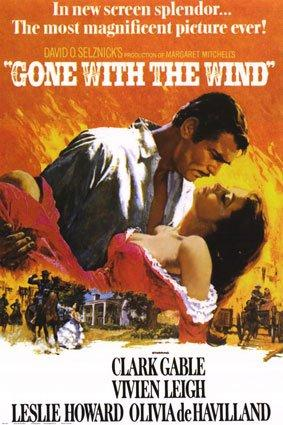
\includegraphics[width=7.5cm]{profClemensSchwender-fig3.jpg}
%    \caption{Most Germans (50+) claim "Gone with the Wind" to be the best movie of all times.}\label{fig3:profClemensSchwender}
%   \end{center}
%\end{figure} 

\begin{figure}
  \begin{center}
    \begin{minipage}[b]{0.40\linewidth}
   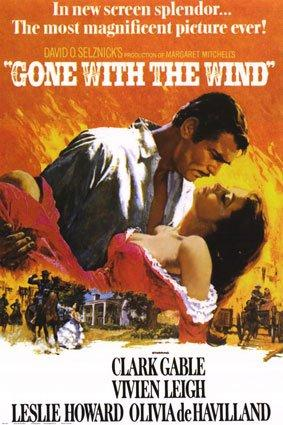
\includegraphics[width=\linewidth]{profClemensSchwender-fig3.jpg}
    \end{minipage}\hfill
    \begin{minipage}[b]{0.55\linewidth}
      \caption{Most Germans (50+) claim "Gone with the Wind" to be the best movie of all times.\label{fig3:profClemensSchwender}}
    \end{minipage}
  \end{center}
\end{figure}


 Preliminary results show that genre preferences change during the lifespan. Preferences change according to age/cohort. Older people favor less aggressive genres like Western, Sciences Fiction or adventure movies. Older people also prefer movies that deal with time periods that they know from their own past experience: Movies about the time and events of World War II are often preferred to movies about contemporary issues. In this category you can find movies like ``The Downfall'' or ``The Boat''. Persons over 70 never mention movies about the future (Science Fiction) as their favorites.

\paragraph{Collaborations}
\begin{itemize}
\item Hochschule f\"{u}r Film \& Fernsehen, Potsdam \\ Dr. Dagmar Hoffmann
\item Universit\"{a}t der K\"{u}nste, Berlin \\ Prof. Dr. Monika Suckf\"{u}ll 
\end{itemize}

\begin{bibunit}[apalike]
\nocite{*}
\putbib[profClemensSchwender4]
\end{bibunit}
